\section{CIG: Computational\\ Intelligence in Games}\label{subsecCIG}

The CIG StarCraft RTS AI Competition is a part of the program of the IEEE Computational Intelligence in Games (CIG) conference since August 2010. In the first year, it failed to determine the winner because of unexpected crashes caused by the custom StarCraft maps. Mike Preuss and his team members organized the event from 2011 to 2013. Traditionally, open-source policy had not been enforced and the maps were unknown prior to the competition day. Since 2014, the Sejong University team (led by Kyung-Joong Kim) has organized the StarCraft AI competition at the IEEE CIG conference. Table~\ref{tableCIG} shows the change of the competition settings over years.  


\begin{table}[h] 
 
 \begin{center}
 \begin{tabular} {| c c c c |}
 \hline
 Year & Tourn. manager & Open-Source & Maps \\
 \hline
 2011 & Manual play & Optional & Unknown \\
 \hline
 2012 & AIIDE TM & Optional & Unknown \\
 \hline
 2013 & Java-based TM & Optional & Unknown \\
 \hline
 2014 & AIIDE TM & Forced & Unknown \\
 \hline
 2015 & AIIDE TM & Optional & Unknown \\
 \hline
 2016 & AIIDE TM & Forced & Announced \\ 
 \hline
 2017 & AIIDE TM & Forced & Announced \\ 
 \hline   
 \end{tabular}
 \end{center}  
 \caption{The running settings of CIG StarCraft AI Competition.}
 \label{tableCIG}
\end{table} 

Since 2010, there have been multiple changes in the selection of tournament management software, open-source policy and map pool announcement policy. The tournament management (TM) software is used to distribute the matches over multiple machines on the network and to automate the competition operation (see the photo in Figure~\ref{figCIGruns}). Although CIG organizers developed their own JAVA-based TM sofware, the AIIDE TM has been used for the competition since 2014~(see details in Section \ref{secTournamentManagerSoftware}). 

Nowadays, the open-source policy is enforced and all the bot source codes are published after the competition. Unlike AIIDE competition, the map pool was not known to the participants before the competition to promote generalization ability of the entries. However, it was found out that participants usually did not exploit the map as a prior knowledge when they prepared the entries. Therefore, the set of competition's maps could be announced in advance. 

\begin{figure}[h]
  \centering
  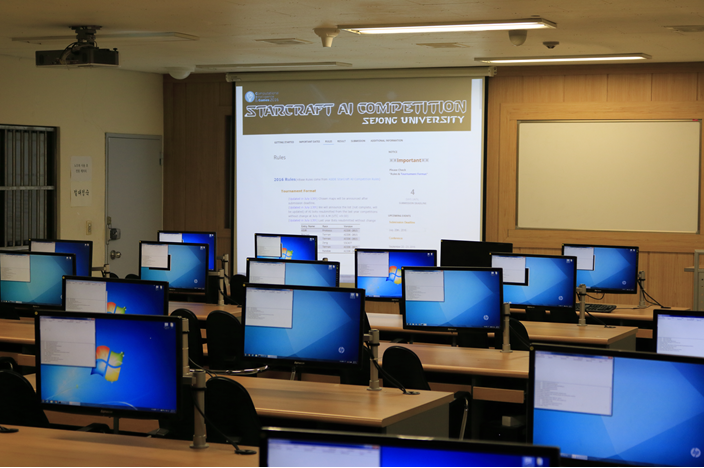
\includegraphics[width=0.5\textwidth]{fig/cig-starcraft-runs.png}
  \caption{In the computing lab, the Tournament Manager software distributes the game matches to multiple machines.}
  \label{figCIGruns}
\end{figure}

\subsection*{CIG 2016 and 2017 Updates \& News}\label{subsecCIGnews}

In 2016 competition, the organizers introduced the two-stage evaluation, where only half of the entries advance to the second stage based on the win ratio of the first stage. The concept of the qualification stage is not new. For example, the simulated car racing competition adopted the two-stage competitions divided into qualification stage and main race \cite{loiacono20102009}. Since StarCraft AI competition is based on the full-round robin tournament, it is important to get high average win ratio against all the opponents. The organizers intended to reduce the chance that the top rankers exploit the low rankers to maximize their win ratio. 

The final stage of the competition consisted only of the games among top rankers (top-8 players) without low-level weak players. Figure~\ref{figCIGtwostages} depicts the change of rankings between the qualification and the final competition stage. We can see that Tscmoo bot replaced Iron bot as the stage winner. 
%It changed the winner of the competition from Iron to TSCMOO but required additional computational resource to run the second stage. 

\begin{figure}[h]
  \centering
  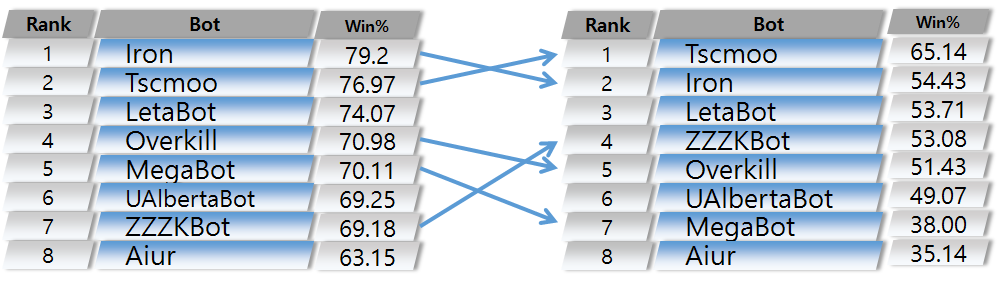
\includegraphics[width=0.5\textwidth]{fig/cig-two-stage-result.png}
  \caption{The change of the rankings between the qualification stage (left) and main competition stage (right).}
  \label{figCIGtwostages}
\end{figure}

The 2016 installment of CIG competition hosted a total of {\em 16 participants}, out of which 9 were new or updated bots and 7 were re-entries from previous year. 
%CIG 2016 competition was divided into two stages: The {\em Qualifying} stage and the {\em Final} stage. The first qualifying stage consisted of Round Robin tournament between all 16 participating bots. 
In total, 11988 round-robin games were played in the qualification stage and 2799 games in the final stage. 
All the games ran on 17 computers for 8 days. 

Any persistent files accumulated by the bots in the qualifying stage were deleted before entering the finals. 
%This stage consisted of 2799 Round Robin games between the 8 bots. 
Best 8 bots, who competed in the final stage were: {\em tscmoo, IronBot, LetaBot, ZZZbot, Overkill, UAlbertaBot, MegaBot} and {\em Aiur}.
The winner of the final stage, {\em tscmoo} bot created by Vegard Mella from Norway, became the overall winner of CIG 2016 tournament with 456 wins and $65.14\%$ win rate in the final stage. Detailed results are depicted in Figure~\ref{figCIGresults}. 

\begin{figure}[h]
  \centering
  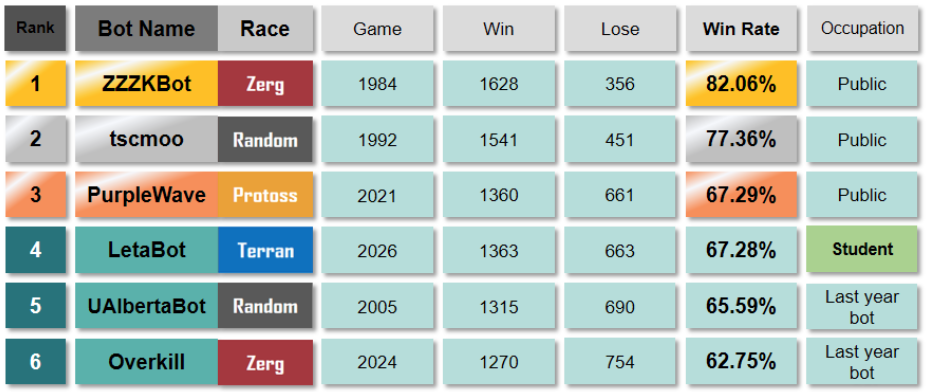
\includegraphics[width=0.5\textwidth]{fig/cig-results.png}
  \caption{Detailed results of the CIG 2016 competition final stage.}
  \label{figCIGresults}
\end{figure}

% CIG 2017 scheduled for Summer 2017
% CIG 2016 happened in Sept. 2016.  
In 2017 competition, the two-stage format was changed back to the single round format. The reason was that the participants did not seem to change their strategy to consider the two-stage tournament. 

{\em Note:} In the future, CIG organizers consider adopting the SWISS-system widely used in the board game community. In this setting, a player does not play against all the other opponents. Instead, the participants are paired with the opponents with similar scores. Such system usually produces the final outcome similar to round-robin with a smaller number of rounds. 

In 2017 CIG competition, organizers tried to increase the number of rounds and finally reached 125 rounds with 190 games per round. Although it required 47,500 games running on 22 machines for two weeks, it allows for a better understanding of the bots' win count dynamics over time. Currently, AI bots often use multiple pre-prepared strategies and adapt them or their selection against specific opponents. Long gameplay experience allows them to learn which strategies are good against which opponents. 
%The file I/O option allows them to save the game experience and reuse them to increase the chance of the wins. 
%For example, Figure~\ref{figureCIGZZZTSCMOO} shows the win counts over multiple rounds for the best (ZZZKBot) and 2nd best bot (tscmoo). It shows that their win counts decrease after around 100 rounds. If we can continue the round-robin after the 125 rounds, the final outcome could be different because other players seem to exploit counter-strategy against the strong players. Figure~\ref{figureCIGMEGASRBOT} shows the change of the win counts for 6th rank (MEGABOT) and 14th ranker (SRBotOne). The MegaBot combined multiple AI players and selectively used them for each opponent. After 100 rounds, their win counts went up to the $75\%$. 
Figures \ref{figureCIGZZZTSCMOO} and \ref{figureCIGMEGASRBOT} depict the win counts of specific bots over time. We can see that the win count tends to increase for some bots and decrease for others - depending on the machine learning approaches they take. 

\begin{figure}[h]
  \centering
  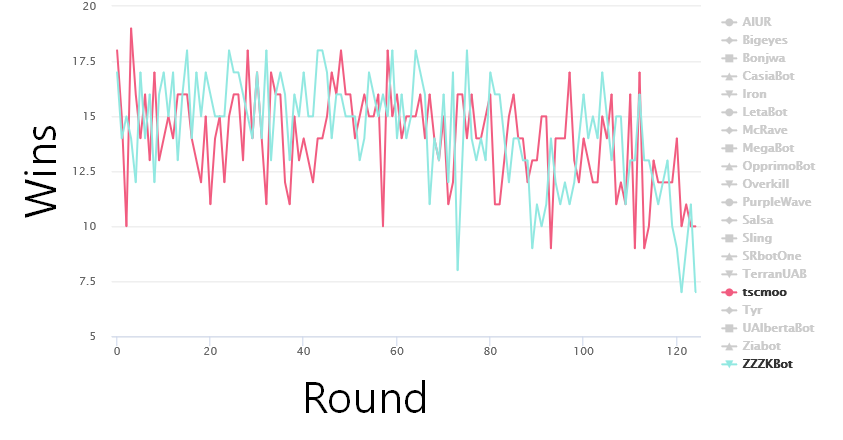
\includegraphics[width=0.5\textwidth]{fig/cig-tscmoo-zzzkbot-winrate.png}
  \caption{The change of win count over multiple rounds for ZZZKBot (1st ranker, blue), and TSCMOO (2nd ranker, red).}
  \label{figureCIGZZZTSCMOO}
\end{figure} 

\begin{figure}[h]
  \centering
  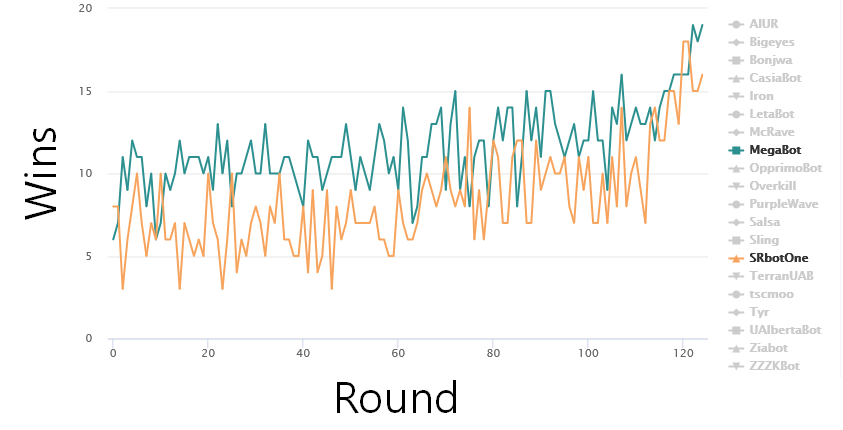
\includegraphics[width=0.5\textwidth]{fig/cig-megabot-srbotone.png}
  \caption{The change of win count over multiple rounds for MegaBot (6th ranker, blue) and SRBotOne (14th ranker, orange).}
  \label{figureCIGMEGASRBOT}
\end{figure} 


% Post-Confererence Event (Man vs. Human Match) 
After the 2017 competition, at 31st of October 2017, Sejong University organized a special event where human players were matched against the AI bots (Figure~\ref{figureSong}). The human players included one novice player (ladder rating around 1100), one middle-level player (around 1500), and a professional gamer, Byung-Gu Song. AI bots in the event were ZZZKBot, the winner of CIG 2017 competition, tscmoo bot, 2nd ranker in CIG 2017, and MJBOT, an AI bot specially designed against human players. The MJBOT has been developed since June 2017 by Cognition Intelligence Laboratory  to beat novice/middle-level human players. 
Each human player played a single game against each AI bot (9 games). 
%In total, there were nine matches (3 human players X 3 AI players). 
The novice human player lost two games against ZZZKBOT and TSCMOO, but won the game against MJBOT, which was not able to finish the game due to the programming bug. In the next session, the middle-level human player lost all three games against the AI bots. Finally, the professional human player Byung-Gu Song managed to win against all the AI bots. This suggests that the AI bots have a potential to compete against novice and middle-level players, but are not yet at the level of professional gamers. All the results and replay files can be found at {\url{http://cilab.sejong.ac.kr/}}. 

\begin{figure}[h]
  \centering
  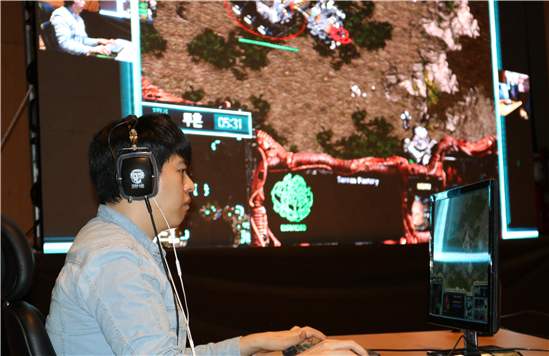
\includegraphics[width=0.5\textwidth]{fig/song_human_ai.png}
  \caption{Professional player Byung-Gu Song playing against AI bots.}
  \label{figureSong}
\end{figure} 
